% Introduction

% Main chapter title
\chapter{Decoding Algorithms} 

% Change X to a consecutive number; for referencing this chapter elsewhere, use \ref{ChapterX}
\label{Chapter3} 

% This is for the header on each page
\lhead{Chapter 3. \emph{Decoding Algorithms}}  

\section{Message Passing Decoding}


The algorithms used to decode LDPC codes are iterative in nature. In every iteration some information has to be passed through the edge of the bipartite graph (Tanner graph), representing corresponding parity check matrix. Thus these type of iterative algorithm are generally termed as message passing decoding\cite{9}.\\
Two type of message passing decoding algorithms are discussed. Bit flipping algorithm takes hard decision at the received information and then principally uses majority whereas belief propagation algorithm uses soft information or the probabilistic approach.\\
LDPC codes are often represented in graphical form by a Tanner graph.
The Tanner graph consists of two sets of vertices.
n vertices for the codeword
bits (called bit nodes), and m vertices for the parity-check equations (called
check nodes).
An edge joins a bit node to a check node if that bit is included
in the corresponding parity-check equation. Number of edges in the
Tanner graph is equal to the number of ones in the parity-check matrix. Notion of Tanner graph was given by Tanner \\
Example:


\[
 H =  \left[ \begin{array} {c|cccccccc} 
  &    B1 &   B2 &   B3 &  B4  &  B5  &  B6  &  B7  &  B8 \\ \hline
c1 &    1  &   1  &   1  &   0  &   0  &   0  &   0  &   0 \\
c2 &    0  &   0  &   0  &   1  &   1  &   1  &   0  &   0 \\ 
c3 &    1  &   0  &   0  &   1  &   0  &   0  &   1  &   0 \\
c4 &    0  &   1  &   0  &   0  &   1  &   0  &   0  &   1 \end{array} \right] 
\]			

\begin{figure}[h!]
\centering
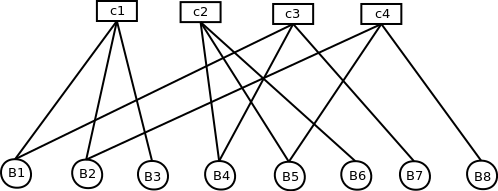
\includegraphics[height=4.5cm,width=10cm]{minSum1}
\caption[Tanner graph]{Tanner graph}
\end{figure}



\subsection{Bit Flipping Decoding} 


 A hard decision is made by the detector for the received bits before passing them to decoder.
Then bits are placed on the bit nodes and passed through the edges of the Tanner graph.
The check node determines that its parity-check equation is satisfied if the modulo-2 sum of the incoming bit values is zero else they pass the flipped value to the corresponding bit.
If the majority of the reception by a bit node are different from its present value then bit node changes (flips) its current value.
This process is repeated until all of the parity-check equations are satisfied, or the decoder gives up.\cite{9}\\
As LDPC matrix is sparse it is unlikely to have same set of checks for a single bit. Still if several checks applied to single bit are incorrect then it is likely to be flipped. \\
\textbf{Example:} \\
If valid codeword for a Tanner graph is c = [0 0 1 0 1 1] (transmitted code); \\
Received code word is y = [1 0 1 0 1 1] (detected code);\\
The decoding algorithm proceeds as following:

\begin{figure}[h]
  \centering
  \begin{minipage}[b]{0.45\textwidth}
    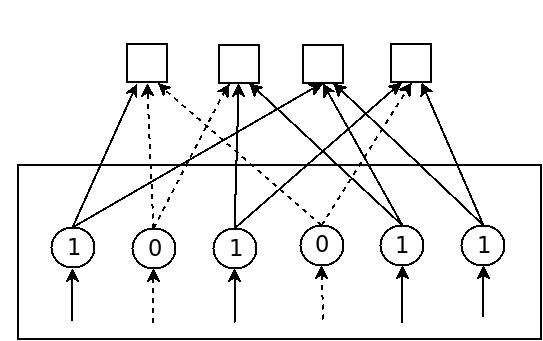
\includegraphics[height=5cm,width=6cm]{initialization}
    \caption[Initializing code bits to bit nodes ]{Initializing bit nodes}
    \label{initialization}
  \end{minipage}
  \hspace{4mm}
  \begin{minipage}[b]{0.45\textwidth}
    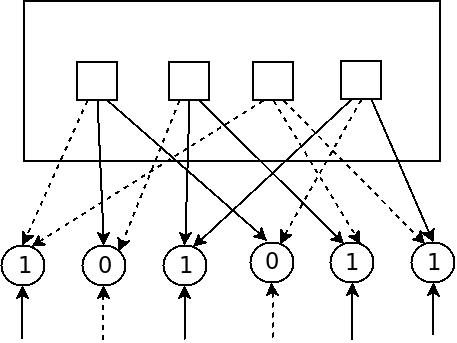
\includegraphics[height=5cm,width=6cm]{PerCheck}
    \caption[Performing computation on check nodes] {Performing computation}
    \label{PerCheck}
  \end{minipage}
\end{figure}    

 \begin{figure}[h]
  \centering
  \begin{minipage}[b]{0.45\textwidth}
    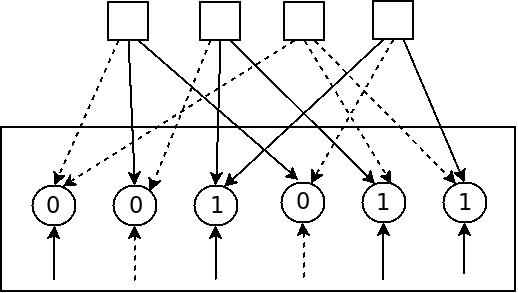
\includegraphics[height=5cm,width=6cm]{BitUpdate}
    \caption[Updating bit node values]{ Updating bit node values }
    \label{BitUpdate}
  \end{minipage}
  \hspace{2mm}
  \begin{minipage}[b]{0.45\textwidth}
    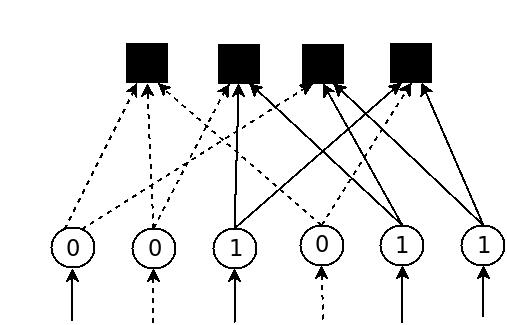
\includegraphics[height=5cm,width=6cm]{Test}
    \caption[Testing for decoding completion]{Testing for completion}
    \label{Test}
  \end{minipage}
\end{figure} 

  
\textbf{Step 1:} The received code bits are assigned to bit nodes in the corresponding Tanner graph, as shown in figure \ref{initialization}. \\
\textbf{Step 2:} Modulo-2 sum is performed at the check nodes. And every bit node gets estimate by all the check nodes connected to it. Every check node send estimate to each bit node connected to it, by computing the result of modulo-2 sum of all the bit nodes connected to it, except the node to which estimate is being send. The computation is illustrated in fig \ref{PerCheck} \\
\textbf{Step 3:} According to the estimates send from check nodes, a bit node take decision by majority. Thus, either is retains its value or flips it, as shown in fig \ref{BitUpdate}.  \\
\textbf{Step 4:} After the iteration, the parity check conditions are checked to satisfy the code word. If code word satisfies all the conditions then decoding stops, else we have to iterate again. \\

\subsection{Belief Propagation Decoding (Sum-Product Decoding)} 


It is soft decision algorithm.
Bit-flipping decoding accepts an hard decision on
the received bits as input, whereas the sum-product algorithm accepts the probability of each received bit as input.
The input bit probabilities are called the a priori probabilities.
The bit probabilities returned by the decoder are called the a posteriori probabilities.
For sum-product decoding these probabilities are expressed
as log-likelihood ratios (LLR).
\begin{align} L(x)=log\dfrac{p(x=0)}{p(x=1)}=log\dfrac{1-p(x=1)}{p(x=1)} \end{align}
 If p(x = 0) $>$ p(x = 1) then L(x) is positive.

Log Likelihood Ratios represent probability as a single value rather than individual probability of being zero and one.
LLR based representation has benefit when probabilities
need to be multiplied LLR need only be added, reducing the implementation complexity.\cite{9}
The goal is to achieve maximum a posteriori probability for each bit. 
The extra information about bit i received
from the parity-check j is called extrinsic information for bit i denoted by $E_{j,i}$. The probability ($P_{j,i}^{ext}$ ) that check j is satisfied when ith bit is one is equal to the probability of having odd number of 1s in the check j other than bit i.
\begin{align} P_{j,i}^{ext} = \dfrac{1}{2}-\dfrac{1}{2} \prod_{i'\in B_j, \ i'\neq i }(1-2P_{i'}^{int})  \end{align}
$P_{i'}^{int}$ is a priori probability of ith bit to be 1. Thus,
\begin{align}
 E_{(j,i)} =  LLR (P_{j,i}^{ext}) = log \left(
\dfrac{1-P_{j,i}^{ext}}{P_{j,i}^{ext}} 
\right)
\end{align}

\begin{align} E_{(j,i)} = log
\left(
\dfrac{\dfrac{1}{2}+\dfrac{1}{2} \prod_{i'\in B_j \ i'\neq i }(1-2P_{i'}^{int}) }{\dfrac{1}{2}-\dfrac{1}{2} \prod_{i'\in B_j \ i'\neq i }(1-2P_{i'}^{int}) } 
\right)
\end{align}

Using relationship: \begin{align}tanh \left(  \dfrac{1}{2}log \left( \dfrac{1-p}{p} \right) \right)=1-2p 
\end{align}

\begin{align} E_{(j,i)} = log
\left(
\dfrac{\dfrac{1}{2}+\dfrac{1}{2} \prod_{i'\in B_j \ i'\neq i }tanh(M_{j,i'}/2) }{\dfrac{1}{2}-\dfrac{1}{2} \prod_{i'\in B_j \ i'\neq i }tanh(M_{j,i'}/2) } 
\right)
\end{align}
where 
\begin{align} M_{(j,i')} =  LLR (P_{j,i'}^{int}) = log \left(
\dfrac{1-P_{j,i'}^{int}}{P_{j,i'}^{int}} 
\right)
\end{align}
Alternatively, using the relationship
\begin{align} 2tan^{-1}(p)=log \left( \dfrac{1+p}{1-p} \right) \end{align}
%%%%%%%%%%%%%%%%%%%%%%%%%%%%%%%%%%%%%%%%%%%%%
Thus extrinsic information from check j to bit i is:
\begin{align} E_{(j,i)} = 2tan^{-1} \left( \prod_{i'\in B_j ,\ i'\neq i }tanh(M_{j,i'}/2) \right) \end{align}
Total LLR passed to bit i is
\begin{align} L_i = LLR(P_i^{int}) = r_i + \sum_{j\in A_i} E_{j,i} \end{align}
where $r_i$ is input a priori for bit i.
But, message sent again from bit nodes to check nodes should avoid the information which checks already have. Thus,
$M_{j,i}$ is not exactly the extrinsic information, it excludes the message generated by the same check node.\\
\begin{align}  M_{j,i} = \sum_{j'\in A_i j'\neq j} E_{j,i} + r_i \end{align}.\\
After every iteration hard decision is made on the LLR post priori. If code satisfies $Hc^T=0$ then decoding stops else $M_{j,i}$ is found and next iteration is performed.

\subsection{Min Sum Decoding}
The min sum decode algorithm is simplification in the sum product algorithm. \\
For BPSK modulation transmitted $0's$ are represented as $-1s$ and transmitted $1s$ are represented as $1s$. \\
The probability that bit 1 is received 
\begin{align} f_y(y|f=-1) = \dfrac{1}{\sqrt{2\pi\sigma^{2}}} \exp{\dfrac{-(y+1)^2}{2\sigma^2}}
 \end{align}
 

The probability that bit 0 is received 
\begin{align} f_y(y|f=1) = \dfrac{1}{\sqrt{2\pi\sigma^{2}}} \exp{\dfrac{-(y-1)^2}{2\sigma^2}}
 \end{align}
 
Thus getting LLR as:
\begin{align}  LLR = \log\dfrac{f_y(y|f=-1)}{f_y(y|f=1)} = \dfrac{-2y}{\sigma^2}
 \end{align}
 
A priori information on the bit node side is expressed in term of LLR as: 
\begin{align}  aPriori[I] = -4 * C[I] * R * \dfrac{Eb}{No} 
 \end{align}
where C[I] = $i^{th}$ code block, R = code rate and 
$\dfrac{Eb}{No}$ = signal to noise power ratio\\
	
Messages are the information propagating from bit nodes to check nodes.
These are initialized to a priori of their respective bit node.	
\begin{align} message[I][J] = aPriori[I] 
 \end{align}
 
Extrinsic information of a bit node is calculated min sum of all the messages connected to 
	that particular check node. 
\begin{align} |E_{(j,i)}| =  Min_{i'\in B_j \ i'\neq i }|M_{j,i'}|   
 \end{align}

\begin{align} sign({E_{(j,i)}}) =  \prod_{i'\in B_j \ i'\neq i }sign(M_{j,i'})   
 \end{align}
 
A posteriori probabilities are the output bit probabilities.
These are used to modify the code block after every iteration.

\begin{align}  aPosteriori[I] = \sum_{j\in A_i} E_{j,i} + aPriori[I] 
 \end{align}
	
Then hard decision is taken on the a posteriori information, that represent the decoded code block.
If decoded code block satisfies $c*H^{T} = 0 $, then decoding stops. Else messages are updated and transmitted back to start the next iteration of decoding.
\begin{align}   message_{(j,i)} = aPosteriori[i] - E_{(j,i)}  
 \end{align}	


